\documentclass[11pt]{article}
\usepackage{icmlko}
\begin{document}

\title{가리면 달라지는데 세어서는 못 맞힌다}
\author{월드모델 실험실}
\date{노트 436 · 2026년 8월 5일}
\maketitle

\begin{abstract}
노트 435가 축을 가리면 grp 이득이 커지는 것을 보이고($-0.0004 \to +0.0152$,
아이돌은 $-0.0921 \to +0.1226$) 한 줄을 덧붙였다 --- \emph{``관측 축 수''가
이제 전이 이득의 예보에 쓰일 수 있다. 노트 411이 못 간 길이 반쯤 열렸다.}
그 반쪽을 쟀다.

\begin{center}
\begin{tabular}{lr}
\hline
관측 축 수 $\leftrightarrow$ grp 이득 (열세 도메인) & $\rho = \mathbf{-0.451}$ \\
집안 열하나만 & $\rho = -0.248$ \\
\hline
\end{tabular}
\end{center}

\textbf{반증됐다}(문턱 $-0.5$). 방향은 맞지만 세기가 모자라고, 그나마도
\textbf{집 밖 둘이 끌고 있다} --- 그 둘은 축이 $5$ 로 묶여 있고 이득이 제일
크다. 집안만 보면 $-0.248$ 이다.

깨는 예가 깔끔하다. \textbf{시장팝업은 축이 셋인데 이득이 $-0.0017$} 이고
\textbf{KR 만화는 축이 다섯인데 $+0.2950$} 이다. 축이 더 적은 쪽이 아무것도
못 번다.
\end{abstract}

\section{인과는 있고 예보는 없다}

두 실험이 같은 것을 말하는 줄 알았는데 아니었다.

\begin{itemize}
\item \textbf{같은 도메인 안에서 축을 가리면} 이득이 커진다 --- 노트 435,
사전 등록 통과. \textbf{가림은 그 도메인의 다른 모든 것을 붙잡아 둔다.}
\item \textbf{도메인끼리 축 수로 견주면} 안 맞는다 --- 여기. 도메인끼리는
축 수 말고도 전부 다르고, \textbf{그 나머지가 더 크다.}
\end{itemize}

노트 411이 걸린 자리와 같은 모양이다. 거기서는 ``관측 축 수 $\to$ 비선형
요구''가 $\rho = +0.781$ 로 섰는데 ``$\to$ 용량 선호''로는 $+0.297$ 로
끊겼고, 노트 412가 축을 실제로 늘려 보니 비선형 요구가 \emph{더 음수}가 되어
그 상관이 인과가 아님을 보였다. \textbf{이번엔 정반대다 --- 인과는 있는데
상관이 없다.}

\section{그래서 예보는 다시 닫힌다}

라벨 없이 셀 수 있는 값으로 새 도메인의 전이 이득을 미리 아는 길은
\textbf{여전히 없다}. 노트 435가 ``반쯤 열렸다''고 적은 것을 \textbf{닫는다}
--- 열린 것은 인과 한쪽이고, 예보는 그 반대쪽이었다.

\begin{tabular}{lp{7.0cm}}
\hline
남는 것 & 가림 실험은 살아 있다. \textbf{새 도메인에 축이 몇 개 붙느냐를
우리가 정할 수 있다면} 그것은 설계 손잡이다 --- 예보가 아니라 \textbf{조작} \\
시장팝업 & 축 셋인데 표지가 아무것도 안 준다. 노트 425가 그 도메인 전용 축을
못 실은 것 · 노트 430이 ``학습에 드는 것의 값 $0.00$''이라 한 것과 한 줄로
읽힌다 --- \textbf{이 도메인은 공유 축에서 아무것도 못 얻는다} \\
집 밖 셋째 & 축이 다섯이 아닌 집 밖 도메인. 두 요인을 가르는 유일한 길 \\
\hline
\end{tabular}

\begin{figure}[h]
\centering
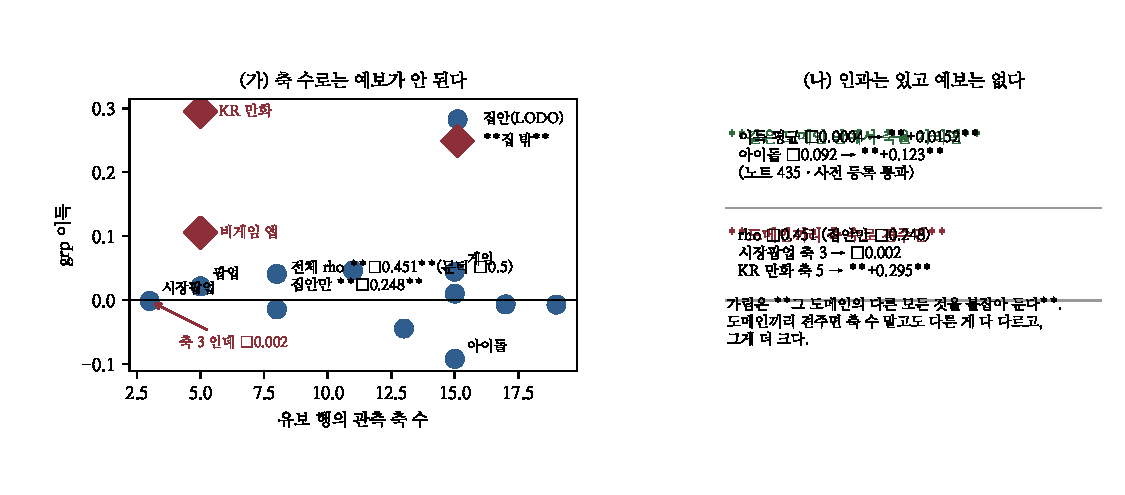
\includegraphics[width=\textwidth]{figs/fig436.pdf}
\caption{(가) 축 수와 이득. 시장팝업(축 3)이 아무것도 못 벌고 KR 만화(축 5)가
제일 많이 번다. (나) 가림은 인과, 셈은 예보 --- 하나만 섰다.}
\end{figure}

\end{document}
